\documentclass{article}
\usepackage[margin=24mm]{geometry}
\usepackage{tikz}
\setlength{\emergencystretch}{3em}
\title{Canonical quadratic norm synthesis with matroid certificates}
\date{Created-at: 2026-10-28 19:49 CET}
\begin{document}\maketitle
\paragraph{Scope.} Deliver the first complete HyMeKo-source to gates path for
the six-input-bit, three-output-bit tower norm over GF(8). Preserve the arbitrary
target XOR contract, all inputs and phase. Audit the published 12/24-bit norm
caches as polynomial functions. Do not claim a full decoder replacement or RL.
\paragraph{Ownership.} Core/Query own compilation and semantic identity. Graph's
existing binary-matroid executable owns weighted basis selection and sparse XOR
coordinates. Its API is not in Quantum's published pinned Graph revision; consume
the existing executable across a hash-recorded JSON boundary without dependency,
Graph source, or provider-policy changes. Quantum validates coefficient
reconstruction and bounded basis independence, emits reversible gates and retains
the generated canonical Core model. Python only authors source and calls native
facades. No alternate parser, IR, matrix solver, matroid engine or simulator.
\paragraph{Implementation.} Extend NativeSynthesis in a quadratic child module
and its existing CLI. Add typed quadratic vocabulary and a generated norm fixture.
The quadratic functions are columns over authored monomial nodes, modulo the
already-live linear input functions. Select output bases and lower their at-most
three-bit linear frames to CNOTs. Compare direct and certified basis emission;
optionally enumerate the bounded one-CNOT input-frame family. Reuse QuantumModel
for gate reading, exact bounded unitary verification and P-graph selection. Raise
its explicit total width limit only from eight to nine for this XOR oracle,
retaining the 64-gate cap. Existing phase specification limits stay unchanged.
\paragraph{Paths and interfaces.} Add synthesis/quadratic.rs, quadratic tests,
Python quadratic source/native adapter and tools/kaggle/quantum\_norm.py; extend
meta\_native, synthesis CLI, lib exports, model width guard and documentation.
Native output contains source/generator identities, canonical generated source,
algebraic witness and selected gate list. Protected items: none. Existing dirty
Geometry/Dynamics/Query changes are preserved. No commits, publication or uploads.
\paragraph{Verification.} Refuse unknown monomials, duplicate algebraic identities,
wrong certificate digest, changed coordinates, singular or incomplete bases and
oversized input. All 512 input/target basis combinations pass independent GF(8)
norm checking, phase probes and round trips in the unchanged native simulator.
Compare with the reviewed public kernel as a separately attributed reference.
Audit cache ranks in the full quadratic function space and modulo linear inputs;
no inferred qubit reduction without a valid erasure/reconstruction schedule.
\paragraph{Budgets and ETA.} Reuse current Transformation checkout at 32c6bb3,
freshly fetched and current. Existing Graph binary is a local integration dependency
with uncommitted source, explicitly recorded; no clean-clone claim. One CPU,
2 GiB and 900 seconds per small native run on Amaterasu, no WSL. At most 31
input frames and existing bounded Graph proposals; record objective counts, not a
timing benchmark. ETA about 60--90 minutes including implementation, targeted
checks and one consolidated report; archive once after writers stop.
\paragraph{Risk and rollback.} Weighted coefficient count is a surrogate, not
the full quantum objective. A public hand-optimized kernel may remain better.
Contraction removes algebraic coordinates, not physical quantum states for free.
Preserve the 883-qubit incumbent. Roll back only this task's named edits/files.
\paragraph{Measured milestone.} The canonical norm compiler and bounded basis
witness validation now run. Direct emission uses 12 Toffolis, weighted basis
emission 11. Reusing the existing phase factorizer and lifting flag-containing
CCZs to Toffolis gives 9; the combined basis/factor schedule also gives 9.
The subsequent shared-product basis gives 6 Toffolis and 34 gates, matching
the public reference's 6 Toffolis with fewer gates (reference: 42). All native
variants passed 512 input/target states; 49 targeted Rust tests and 3 Python
tests pass. The 12/24-bit raw caches have full ranks 10/21 even after quotienting
by the live linear inputs. Optional input-frame enumeration was not needed for
this milestone. Inverse synthesis and broader factor discovery remain next.
\paragraph{Continuation at 20:16 CET.} Extend the same quadratic compiler to
shared rank-one products. Seven symmetric GF(8) parity-product candidates form
a rank-six column family; Graph chooses a basis. Authored output decompositions
are verified against their monomial coefficients and reconstructed through the
Graph witness. Emit each selected product into its output parity vector using
reversible CNOT frames and one Toffoli, with no stored product ancilla. Bound the
witness rank to six (64 XOR sums for independent checking), still at most nine
physical qubits and 64 gates. This tests an own algebraic route to the public
six-Toffoli count; it is not an RL experiment or a full decoder change.
\begin{center}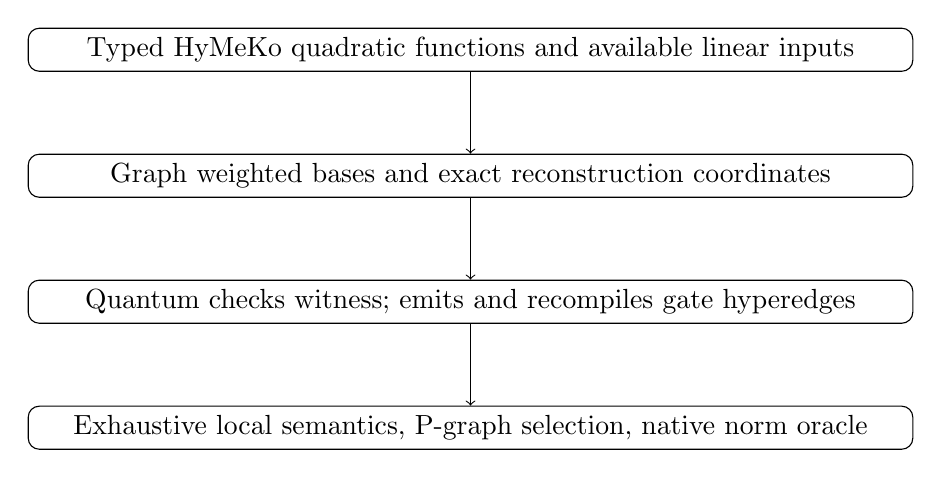
\begin{tikzpicture}[every node/.style={draw,rounded corners,align=center,text width=11cm},node distance=16mm]
\node (a) {Typed HyMeKo quadratic functions and available linear inputs};
\node (b) [below of=a] {Graph weighted bases and exact reconstruction coordinates};
\node (c) [below of=b] {Quantum checks witness; emits and recompiles gate hyperedges};
\node (d) [below of=c] {Exhaustive local semantics, P-graph selection, native norm oracle};
\draw[->] (a)--(b);\draw[->] (b)--(c);\draw[->] (c)--(d);
\end{tikzpicture}
\end{center}
\end{document}
